\documentclass[a4paper, 11pt]{report}
%\usepackage{fancyvrb}
%\usepackage{color}

\renewcommand{\bibname}{References}
\bibliographystyle{ieeetr}

\usepackage{sectsty}
\usepackage[margin=1in]{geometry}
%\usepackage[onehalfspacing]{setspace}
\usepackage[pdftex]{graphicx}
\usepackage{subfig}
\usepackage{wrapfig}
\usepackage{tikz}
\usepackage{amsmath}
\usepackage{bm}
\usepackage{hyperref}
\usepackage{appendix}

\hypersetup
{  colorlinks=true,        % colored links, not boxes
   linkcolor=blue,         % internal links
   citecolor=red,          % bib links
   filecolor=magenta,      % file color
   urlcolor=cyan           % external color
   %linkcolor=black,         % internal links
   %citecolor=black,          % bib links
   %filecolor=black,      % file color
   %urlcolor=black           % external color
}
\usepackage{url}
\usepackage[square, comma]{natbib}
%\usepackage[english]{babel}
\usepackage{float}

\setlength{\parindent}{0pt}
\linespread{1.3}

% tikz
\usetikzlibrary{arrows}
\usetikzlibrary{snakes}
\usetikzlibrary{patterns}
\usepackage{listings}

\lstset{ %
language=c, 	                % choose the language of the code
basicstyle=\scriptsize,	        % the size of the fonts that are used for the code
numbers=left,                   % where to put the line-numbers
numberstyle=\scriptsize,        % the size of the fonts that are used for the line-numbers
stepnumber=1,                   % the step between two line-numbers. If it's 1 each line will be numbered
numbersep=20pt,                 % how far the line-numbers are from the code
backgroundcolor=\color[rgb]{0.9,0.9,0.9},  % choose the background color. You must add \usepackage{color}
showspaces=false,               % show spaces adding particular underscores
showstringspaces=false,         % underline spaces within strings
showtabs=false,                 % show tabs within strings adding particular underscores
frame=single,                   % adds a frame around the code
tabsize=4,                      % sets default tabsize to 2 spaces
captionpos=b,                   % sets the caption-position to bottom
breaklines=true,                % sets automatic line breaking
breakatwhitespace=false,        % sets if automatic breaks should only happen at whitespace
escapeinside={\%*}{*)}          % if you want to add a comment within your code
}

\begin{document}
    {
    \pagestyle{empty}       % no page numbers
    \begin{titlepage}
\label{pg:title}
\begin{center}
\vspace*{0.5in}
{\bf \Huge Design and Stabilization of a}\\[0.25in]
{\bf \Huge One Legged Hopping Robot}\\[0.5in]
{\bf \Large B.Tech. Project}\\[0.25in]
{\normalsize \it of}\\[0.25in]
{\bf \Large Pratik Chaudhari}\\[0.2in]
{\bf \Large Roll No. - 06D01015}\\[0.8in]
{\bf \Large under the guidance of}\\[0.2in]
{{\bf \Large 	Prof. Hemendra Arya}\\
{\normalsize	 Department of Aerospace Engineering, IIT Bombay.}}\\[0.25in]
{\normalsize \it and}\\[0.25in]
{{\bf \Large Prof. Bhartendu Seth}\\
{\normalsize	 Department of Mechanical Engineering, IIT Bombay.}}\\[1in]
\includegraphics[scale=0.2]{fig/iitblogo.pdf} \\
Indian Institute of Technology Bombay\\
\today
\end{center}
\end{titlepage}


    \newpage
\vspace*{0.75in}
\label{pg:certi}
\begin{center}
{\bf \Huge Certificate}\\[0.5in]
\end{center}
{\normalsize This is to certify that this report of {\bf Pratik Chaudhari} on the topic, {\bf Design and
Stabilization of a One Legged Hopping Robot} towards partial fulfilment of the requirements of {\bf B.Tech.
Project AE 497}
is approved by me for submission. It represents the work carried out by the student under my guidance.}\\[1in]

\begin{center}
{\bf \large Prof. Hemendra Arya} \hspace{1.2in}{\bf \large Prof. Bhartendu Seth}\\[0.1in]
{\normalsize Guide \hspace{2.9in} Co-guide\\[0.1in]}
\end{center}


    \thispagestyle{plain}
\abstract
Single-legged locomotion gait is a hopping motion consisting of alternate flight and stance phases. In such a hopping robot, if the energy lost in friction and impacts is compensated, then control of robot attitude can result in stable hopping motion. In this regard, use of a reaction wheel mechanism as an attitude control actuator is a novel and energy efficient approach.\\

This report discusses the development of the mechanical and electronic systems of a one legged hopping robot. An energy efficient mechanism has been fabricated for experiments to demonstrate a stable running gait as well as in-place hopping using SLOM concept. A test-rig was also built to pivot the robot near its C.G. to perform attitude orientation experiments independently of hopping. Electronics developed during the course of this project consists of an onboard controller, DC motor drivers using MOSFETs and an inertial measurement unit.\\

Dynamics of impulsive systems is significantly different due to its hybrid nature and hence a detailed model of the hopping robot was formulated to study it. This involved simulations for a running gait, in-place hopping as well as exercises in finding the stability basin of the hopper design. Controllabilty of non-linear systems and optimal control techniques were also studied to be implemented later.\\

A full-state attitude feedback system was developed using inertial sensors since the hopping system does not have physical contact with any fixed reference during the flight phase. A kalman filter was designed to attain drift free orientation feedback and was implemented in a real-time embedded controller.

\vspace{1cm}
\begin{description}
  \item[Keywords:] SLOM, offset-mass, reaction wheel, hopping robot, non-linear hopping gait model, inplace hopping, poincare map, attitude control, PID, kalman filter, inertial sensors.
\end{description}
    }
    {
    \newpage
    \addtolength{\topmargin}{-1in}
    \pagenumbering{roman} \setcounter{page}{0}
    \tableofcontents
    }
        
    \newpage
    \addcontentsline{toc}{chapter}{List of figures}
    \label{pg:figlist}
    \listoffigures

    \pagenumbering{arabic} \setcounter{page}{1}
    \pagenumbering{arabic} \setcounter{page}{1}
\chapter{Introduction}
\label{chap:intro}
This is a test.

    %\chapter{Problem Statement}
\label{chap:problem}
This chapter discusses previous work on the one legged hopper at IIT Bombay and formulates the exact problem statement and the scope 
for this project.

% 1. sayyad
%     poincar`e map ... read his abstract
%     saboo...sanmukh
% 2. londhe
%     describe mechanism
% 3. simit
%     contributions
% 4. siraj
%     contributions
\section{Previous work}
\subsection{1-D Hopper}
Vitthal Londhe~\cite{londhe} developed a 1D hopper and demonstrated in place hopping capabilities. The design was aimed at minimizing
the energy losses and making the robot easy to assemble and disassemble.
\begin{wrapfigure}{r}{0.4\textwidth}
\centering
\includegraphics[scale =1.5]{fig/londhe.pdf}
\caption[Vertical Hopper]{Vertical Hopper \cite{londhe}}
\label{fig:2_londhe}
\end{wrapfigure}
Fig.~\ref{fig:2_londhe}, shows the major parts of this hopper viz. a winding motor with the energy pumping mechanism and a telescopic 
leg with a ratchet and paul constraint. The hopper is also confined to a fixed vertical axis. The leg is connected to a compression 
spring. A motor is used to compress this spring.\\

The constraint mechanism consists of a bell crank attached to the paul so that when the leg impacts upon the ground, the paul comes 
free of the ratchet teeth and the spring is free to compress further. This is the first use of impact forces for releasing the energy 
pumping mechanism in a one legged hopper. Thus the motor does not need to do work against the spring force to hold the leg in the compressed position. The latch mechanism mechanically latches the leg in place and unlatches it only when the leg touches the ground.
\subsection{SLOM Hopper}
Fig.~\ref{fig:2_hop2d} shows the prototype developed by Sharma and Gebretsadik~\cite{londhe} for which Vipul Saboo~\cite{saboo} 
designed and fabricated the EPM for it. He could also demonstrate hopping of the robot without active balancing.

The robot consists of a body and a telescopic leg of rectangular cross-section attached to the body by a spring. The leg also has a 
freely rotating ankle with a foot attached to it. The ankle ensures that the foot always falls flat on the ground irrespective of the 
orientation of the robot while touchdown.\\
\begin{figure}
\centering
\subfloat[SLOM hopper : sketch]{\includegraphics[scale = 1.5]{fig/saboo.pdf}\label{fig:2_hop2d}}
\hspace{1in}
\subfloat[Paul and ratchet]{\includegraphics[scale = 1.2]{fig/ratchet.pdf}\label{fig:2_ratchet}}
\caption[2D SLOM hopper]{2D SLOM hopper \cite{saboo}}
\label{fig:2_saboo}
\end{figure}
To reduce the friction between the telescopic leg and the body, teflon bearings are used in sets of two on each of the four sides of 
the leg. The construction of the robot makes it very difficult to assemble and disassemble it. Also, the mass of the leg is almost 
${2/3}^{rd}$ of the mass of the body which results in huge energy loss of the system during impacts.
The EPM consists of a ratchet and a pawl with a voice-coil which activates the pawl. The voice-coil is electrically actuated by a 
mechanical limit switch attached on the foot of the robot. There is also a latch-type EPM where the motor can be switched off after 
the spring is compressed.\\

Simit \cite{simit} developed a treadmill and constraining mechanism (TCM) for the SLOM hopper. He also demonstrated an embedded system
for hopping height control using a feed-forward and PID controller. A ground station for gathering telemetry data from the TCM 
interface.

\subsection{Reaction wheel}
Siraj \cite{siraj} modeled attitude control of the hopper as a position control problem for the reaction wheel pendulum. He
demonstrated PID and LQR control strategies for the reaction wheel pendulum. Optimal control strategies have to be looked into because
as observed by Beuhler \cite{Bue_PassRun, ARLMono2}, almost 50\% of the total energy is utilized in swinging the leg mass i.e. in
attitude reorientation. A inertial measurement unit (IMU) using a complementary filter was also developed.

\section{Problem formulation}
The SLOM hopper was used as a test bed for devising hopping strategies by Saboo \cite{saboo}, Simit \cite{simit} and Siraj \cite{siraj}. However, it was an over-designed system with large energy losses due to impacts and friction. It was necessary to
remove these flaws in the robot before further work could be done on it. Hence, it was decided to go ahead with a completely new
mechanical design for the hopper keeping the following things in mind about the previous design.
\begin{enumerate}
\item
SLOM concept is quite novel and the new design will be based on it.
\item
Compression spring need an enclosure outside them to keep them in place when in compression. This results in frictional losses in
every cycle of energy pumping. Tension springs on the other hand do not have such frictional losses associated with them. It was thus
decided to use tension springs for the new design.
\item
The SLOM hopper could not hop above a height of 10 cm. The energy pumping mechanism (EPM) was the limiting factor. For achieving heights larger than this, we need to significantly reduce the leg mass and have a more energy efficient EPM.
\item
A reaction wheel should be present on the hopper and this will be used to reorient the robot to demonstrate both in-place hopping
and running capabilities.
\item
An embedded system along with on-board power supply shall be used to control the actuation, sensors and execute the control law.
\end{enumerate}



    \chapter{Robot Design}
\label{chap:mech_design}

The final design of the hopping robot is described in this chapter. We first look at two previous designs devised to make use of SLOM effect. After ironing out some deficiencies, we arrive at a simplistic design that satisfies our criteria.
\begin{figure}[H]
\centering
\subfloat[Design 1]{\label{fig:3_design1} \includegraphics[width=0.5\textwidth]{fig/design1.pdf}}
\subfloat[Design 2]{\label{fig:3_design2} \includegraphics[width=0.5\textwidth]{fig/design2.pdf}}
\caption{Previous hopping robot designs : Approx. height = $500\;mm$}
\label{fig:3_prevdes}
\end{figure}

\section{Mechanical}
\subsection*{Previous Designs}
\label{sec_3:mechanical}

A description of the two designs is given in the report for Stage I \cite{stage1}. The evaluation 
of these two designs is as follows,
\subsubsection*{Design 1}
\begin{enumerate}
  \item
  It has to be ensured that the winding winch does not slip over the pulley when the platform is suddenly released from the constraint. At the same time, the winch must be free enough so as not to hinder the 	movement of the platform after the release.
  \item
  The platform moves over the leg with the help of a circular bushing. There is another bushing for the lower leg to move into the upper leg. These circular bushings are light and durable.
  \item
  The hatch that is a crucial part of the energy release and the constraint mechanism is the weakest part, but it can break easily.
\end{enumerate}

\subsubsection*{Design 2}
\begin{enumerate}
 \item
The sleeve of the motor is kept on the same side as that of the reaction wheel and helps to provide an offset mass for the SLOM effect. Body mass also helps to obtain an offset C.G.; thus the distance of the reaction wheel from the axis need not as be as large as calculated in the adjoining analysis.
\item
The worm-worm wheel on the rack mechanism provides a huge mechanical advantage and thus reduces the maximum torque required from the motor. This scales down the mechanical system as well as the electronic system requirements.
\item
All the force of the extension springs is coming as an axial load on the shaft of the motor. We thus
need to choose a gearbox that can handle these axial loads.
\item
The friction pulley has to work against the pual spring, sleeve spring and the horizontal component of the rack force ($k\:x\:tan\:\theta$) to keep the string in tension. This is compounded by the fact that the there is a maximum $\omega$ the motor can
accelerate to in the energy storing phase. It is much better if this $\omega$ is dictated by the torque requirements which are as
critical rather than this mechanism.
\item
Less resolution on the desirable extension of springs because we are operating on a rack. This can however be easily taken care of in the pitch control law.
\item
The constraint mechanism for Design 2 is not reliable enough and should be improved upon. The major problem is to provide an opposing force to the horizontal component of the rack--worm-wheel force ($k\:x\:tan\:\theta$). This force has to be present when the motor is extending the springs and should be removed before we release the ratchet so that the platform along with the motor-sleeve is free to move up. To disengage the motor from the rack, the spring shown in the left part of Fig. \ref {fig:3_design2} will have to be there as well.
\end{enumerate}

\subsection*{Final solution}
Both the designs given in Section \ref{sec_3:mechanical} had significant drawbacks and hence a newer design was made utilizing their individual mechanisms and the knowledge gained from analyses.

The salient features of this design are as follows,
\begin{enumerate}
  \item 
  As shown, in the figure, it consists of two large flanges with all the components arranged inside it. Enclosing the components inside the flanges makes it a compact, closed system with only essential components like batteries, motors, circuit boards being accessible from outside.
  \item
  One major component of this design is the rack and pinion mechanism. It is difficult to cut a 45 degree rack due to fabrication constraints. However, this mechanism has been built and fixed on the robot successfully.
  \item
  The whole robot is built in such a way that it can be pivoted fully near its C.G. to a test--rig. This test--rig simply consists of two large columns from which the robot hangs. It is a simple contraption and should prove handy while performing experiments on the robot.
  \item
  The ratchet and paul mechanism is on the same axis as the band drive. There is a servo motor on the outer side near the paul to actuate it (which is not shown here).
  \item
  Another servo motor sits on the vertical portion of the robot to ensure that the motor sleeve gets detached after extending the spring.
  \item
  We have ensured that the C.G. of the system lies along its centerline and hence there are no lateral moments. This is done by putting batteries on the opposite side of the reaction wheel motor.
\end{enumerate}

\begin{figure}[!htp]
\centering
\includegraphics[scale=0.8]{fig/hopper_detach.png}
\caption[Solidworks hopping robot assembly]{Solidworks hopping robot assembly : Motor sleeve, reaction wheel and rack and pinion. Note that one of flanges is hidden in the picture to see the internal components}
\label{fig:3_solidworks1}
\end{figure}

\section{Analyses}
\label{sec_4:analyses}
We need to find approximate design estimates of the hopping robot by performing analysis. The following three values are what we are interested in.
\begin{enumerate}
\item
Masses of the platform and the leg
\item
Dimensions of the reaction wheel based on the above masses
\item
Choice of winding and reaction wheel motors
\end{enumerate}

\subsection*{$2$ mass problem}
\begin{figure}[!htp]
\centering
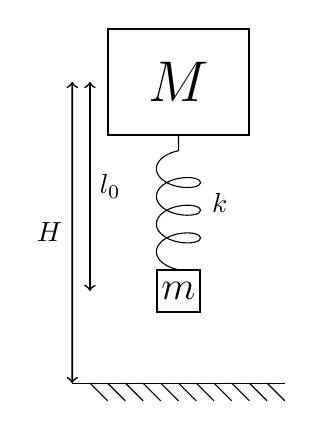
\begin{tikzpicture}[scale=0.45]
\draw (-3,0) -- (3,0);
\foreach \x in {-2.5,-2,...,2.5}
\draw (\x,0) -- (\x+0.5,-0.5);

\path (-2,7) coordinate(M1);
\path (2,10) coordinate(M2);
\path (-0.6,2) coordinate(m1);
\path (0.6,3.2) coordinate(m2);

\draw [thick](M1) rectangle (M2) node[midway]{\huge{$M$}};
\draw [thick](m1) rectangle (m2) node[midway]{\Large{$m$}};

\path (-2.5,0) coordinate (O);
\path (-2.5,2.6) coordinate (SPL);
\path (-2.5,8.5) coordinate (H);

\draw[<->] [semithick](O)++(-0.5,0) -- (-3,8.5) node[midway, left]{$H$};
\draw[<->] [semithick](SPL) -- (H) node[midway, right]{$l_0$};

\draw[snake=coil, segment amplitude=8pt] (0,3.2) -- (0,7) node[midway,right=2ex]{$k$};
\end{tikzpicture}
\caption[2 mass problem]{2 mass problem \cite{simit}}
\label{fig:3_2mass}
\end{figure}
The basic idea behind a hopper is like that of the 2 masses connected by a spring problem. If the system shown in Fig.
\ref{fig:3_2mass} is allowed to fall from a height, the heavier mass pulls the smaller mass with it back into the air
after impact. Every cycle is accompanied by a loss in energy due to the inelastic impact of the smaller mass with the
ground. If we pump this energy back into the system using an external agent in every cycle, we can ensure sustained hopping at the chosen height. The 2 mass problem can thus be taken as a basis to compute the range of values of masses for acceptable performance. It is seen from Fig. \ref{fig:3_2mass} that if $h_i$ are progressive heights, we have the relation,
\begin{equation}
h_n = \frac{Mh_{n-1} + ml_0}{M + m}
\end{equation}
\begin{equation}
\label{eqn:3_eloss}
E_{loss} = \frac{Mg\;(H-l_0)}{1 + M/m}
\end{equation}
\begin{figure}[!htp]
\centering
\includegraphics[scale=0.6]{fig/2mass_m.pdf}
\caption{Torque variation with m}
\label{fig:3_torque2mass}
\end{figure}

Fig. \ref{fig:3_torque2mass} shows the required torque  for extending springs to compensate the energy 
lost during impact fully within 0.2 sec. It is observed that m is the single most important parameter in 
hopper design. The required torque is a very strong function of the leg mass. As this mass increases, we 
need a larger motor to satisfy torque requirements. It is noted that a value of about 0.4--0.6 kg
can be called a reasonable estimate for the leg mass as we can easily choose a motor delivering the 
required torque for these values.\\

It is also seen that an extension of about 11 cms with a single spring of k = 300 Nm is needed to 
compensate the energy loss for hopping heights of 80 cms. So we should ensure that we can provide a 
maximum extension around 15 cms.

\subsection*{Impact Analysis}
The desired hopping height dictates a hopping frequency. Intuitively, smaller hopping height results in 
large number of impacts per time and consequently in larger energy loss per unit time. This is seen from 
Fig. \ref{fig:3_freq_height} because the hopping frequency is closer to the natural frequency for small 
hopping heights. However, beyond this consideration, since the hopper is a spring mass system, it 
possesses a natural frequency of its own. If the hopping frequency is near to this natural frequency, a 
large amount of energy is taken away by impact forces in every cycle. We intend to arrive at a range of 
values for the masses to ensure a large difference between the hopping frequency ($\omega_{hop}$) and the 
natural frequency ($\omega_{nat}$).
\begin{figure}[!h]
\centering
\subfloat[Freq. variation with height]{\label{fig:3_freq_height}\includegraphics[width=0.5\textwidth]{fig/freq_hopheight.pdf}}
\subfloat[Freq. variation with m]{\label{fig:3_freq_m}\includegraphics[width=0.5\textwidth]{fig/freq_m.pdf}}
\caption{Impact Analysis : Frequency variation}
\label{fig:4_freq_var}
\end{figure}
Fig. \ref{fig:3_freq_m} succinctly depicts all the above analysis. As the leg mass increases, the hopping frequency goes closer to the natural frequency i.e. more impact per unit time. To compound matters, more and more energy is lost per impact. So the conclusion from impact analysis is that the leg mass should be as low as possible. It is also seen from Fig. \ref{fig:3_freq_m} that \mbox{m = 0.4 -- 0.6 kg} is a good solution as well as an achievable one. 

\subsection*{Reaction Wheel}
For achieving a running gait with the hopper, it has to be started with the exact initial pitch and 
horizontal velocity. For any other initial condition, the hopper is pitch unstable and will not be able to 
continue the running gait. As mentioned in \cite{shanmug}, an offset mass acts as a passive stabilization 
to the pitch attitude of the hopper. To get rid of this need for exact initial condition which is quite 
impractical, we design a reaction wheel on the hopper. This will result in torque coupling on the pitch 
axis and thus provide an active control over the pitch of the robot.\\

We consider the case where the pitch is such that we have no horizontal velocity and no stabilization impulse from the ground. This pitch is reoriented to 30 degrees within one hop which corresponds to a huge horizontal velocity of 13.5 m/s. The stable pitch will be less than this for lower velocities. In actual operation
there will be large reaction wheel torques only while converting the initial condition into a stable
running gait. After that there will only be small control torques about the stable pitch angle.
\begin{figure}[!h]
\centering
\includegraphics[scale=0.4]{fig/rewac_radius.pdf}
\caption{Torque requirements vs radius}
\label{fig:3_rewac_torque}
\end{figure}
Figs. \ref{fig:3_rewac_torque} has been plotted for distance of C.G. = 6 cms and radius of the reaction wheel taken as 6 cm (mass = 1.5 kg) after a similar analysis for variation in CG. We can see that the required torque for reorientation as mentioned in above is around 500 mNm with output power being around 1.5 W.

\section{Components}
\subsection*{Motors}
\begin{description}
 \item[\textsf{Reaction wheel motor}]
  3257CR024 motor is chosen with a standard gear box of 14.4 : 1. The stall current is below 5A and can be easily handled with the motor drivers designed using MOSFETs with 512 cpr encoders.
  \item[\textsf{Spring extension motor}]
  We take common values of worm-worm wheel diamter ratio (0.5), pressure angle (20 deg), helix angle for 
  worm (25 deg) and co-efficient of friction $\mu = 0.3$. The torque required from the motor is not more 
  than 200 mNm. The total power required for this task is about 4.5 W. We choose the 2342CR024 motor 
  for this task. The gear box is taken as a 43 : 1 with 512 cpr encoders.
  \item[\textsf{Servo 3003}]
  This is used for the ratchet and paul mechanism as well as the motor sleeve disengagement. The torque requirements are satisfied easily since not much torque is needed.
  \item[\textsf{Motor Driver}]
  The stall current of both the motors is near 5A and hence a conventional readymade H-bridge will not work. I designed a H-bridge using MOSFETs (CSD 16404) and MOSFET drivers (TPS 2836) to provide good drive to the motors with a maximum current of 21A and $R_{GS} =$ 4.1 $\Omega$. It can be controlled using just two microcontroller pins.
  \begin{figure}[H]
  \centering
  \subfloat[Top side]{\includegraphics[width=0.35\textwidth, angle=90]{fig/hbridge_top.png}}
  \subfloat[Bottom side]{\includegraphics[width=0.35\textwidth, angle=90]{fig/hbridge_bot.png}}
  \caption{MOSFET Hbridge}
  \label{fig:3_hbridge}
  \end{figure}
  \end{description}

\subsection*{Inertial Measurement Unit}
\begin{description}
  \item[\textsf{Accelerometer - ADIS 16201}]
  Provides 14-bit signed readings. The accelerometer has a sensitivity of 2.162 LSB/mg with a noise of 22 
  LSB. The accelerometer also consists of an inclinometer to measure the angle with respect to the ground. 
  However, it provides a sensitivity of only 10 LSB/deg. This necessitates the need of onboard inverse 
  tangent tables to get the pitch angle from accelerometer readings. The bandwidth of the accelerometer is 
  2.25 KHz.
  \item[\textsf{Single Axis Gyroscope - ADIS 16255}]
  Provides 14-bit signed readings with internal temperature calibration. The sensitivity of the gyroscope 
  is $0.07326$ $^o/$s/LSB for the whole range of $\pm\;320$ $^o/$s with a noise of $0.48$ $^o/$s.  The 
  bandwidth of the gyroscope is 50 Hz which severely limits the update rate of the filter.
\end{description}

\subsection*{Computing}
\begin{description}
  \item[\textsf{Microcontroller}]
  Microchip dsPIC33F64MC804 can run at 40 MIPS with an onboard flash memory of
  64 KB along with a 16 KB SRAM. There are a host of integrated peripherals like Serial Peripheral 
  Interface (SPI), UART, Analog to Digital converter (ADC), Quadrature Encoder (QEI) and timers to 
  generate Pulse Width Modulation (PWM) that can be used for motor control. Pickit 2 is the USB programmer 
  used to program the flash of the microcontroller.
  \item[\textsf{XBee Modules}]
  Used to provide a wireless link between the embedded system and the PC with the help of a custom made 
  FT232 USB-UART converter. This is a major tool for all debugging and grabbing telemetry.
  \begin{figure}[H]
  \centering
  \subfloat[Top Side]{\label{fig:3_brddoctop}\includegraphics[width=0.49\textwidth]{fig/rewac_top.pdf}}
  \subfloat[Bottom Side]{\label{fig:3_brddocbot}\includegraphics[width=0.49\textwidth]{fig/rewac_bot.pdf}}
  \caption{On-board controller pinouts}
  \label{fig:brddoc}
  \end{figure}
\end{description}
Fig. \ref{fig:3_brddocbot} and \ref{fig:3_brddoctop} show the onboard controller that was used for the experiements. A new board incorporating all drives and motors has been designed but not fabricated yet.













    \chapter{Hopping Gait}
\label{chap:hopping_gait}

We plan to generate a stable hopping gait by utilizing the SLOM concept for the system designed in Chapter. 
\ref{chap:mech_design}. The strategy to do that would be to first derive the equations of the motion of the 
whole system and propagate them using correct constraints and event solvers. The initial part of this 
chapter addresses these issues. Once we can propagate these set of equations from any initial condition, we 
try to find a relation between the impact states of every hop. The variation of these impact states will 
enable us to find if the gait is stable or not. We will try to find out good sets of initial conditions 
such that the impact states do not change much i.e. impact states are the fixed point of the Poincare Map 
of the set of differential equations.\\

Next step in the analysis would be to devise a control strategy for attitude re--orientation. The spring 
extension controller is already devised while finding the impact states.

\section{Euler-Lagrange equations}
\begin{figure}[!htp]
\centering
\includegraphics[scale=0.30]{fig/line_sketch.pdf}
\caption{Line sketch for the hopper}
\label{fig:4_line_sketch}
\end{figure}

We use the Euler--Lagrange equations derived from the Lagrangian as follows,
\begin{equation}
 T \:=\: \frac{1}{2}\:\:\left[\:\:m_w\:(\:\dot{x_w}^2 + \dot{y_w}^2\:) + m_p (\:\dot{x_p}^2 + \dot{y_p}^2\:)
  + m_l\:(\:\dot{x_l}^2 + \dot{y_l}^2\:) +  J_w\:(\:\dot{\phi} + \dot{\theta}\:)^2
  + J_b\:\dot{\theta}^2\:\:\right]
\end{equation}
\begin{equation}
V\:=\: g\:\left[\: m_l\:y_l\:+\: m_w\:y_w\:+\: m_p\:y_p\:\right] + \frac{1}{2}K\:(l - l_0)^2
\end{equation}
%\begin{equation}
% L = T - V
%\end{equation}
where,
\begin{eqnarray*}
x_l(t) &=& x(t) + \left[\:d - (\:l(t)- h\:)\:\:\tan \theta\:\right]\cos \theta\\
y_l(t) &=& x(t) + \left[\:l(t) - h \right]\:\:\cos \theta + d\:\:\sin \theta\\
\\
x_w(t) &=& x(t) - \:(\:d_w - d\:)\: \cos \theta\\
y_w(t) &=& y(t) - \:(\:d_w - d\:)\: \sin \theta
\end{eqnarray*}
\begin{eqnarray*}
x_p(t) &=& x(t) + d\: \cos \theta\\
y_p(t) &=& y(t) + d\: \sin \theta
\end{eqnarray*}

\vspace{0.2in}
\begin{tabular}{l @{ : } l}
$x_w$, $y_w$ & co-ordinates of the reaction wheel\\
$x_l$, $y_l$ & co-ordinates of the C.G. of the leg\\
$x_p$, $y_p$ & co-ordinates of the platform\\
$x$, $y$ & co-ordinates of the C.G. of the whole robot\\
$l(t)$ & length of the spring\\
$\theta$ & pitch angle measured as shown in the figure\\
$\phi$ & angle rotated by the reaction wheel relative to the robot\\
$d$ & distance of C.G. from the line of impact force\\
$d_w$ & distance of reaction wheel from the line of impact force\\
$l_0$ & non--extended length of the spring
\end{tabular}
\vspace{0.2in}

For co-ordinates of $q = \left[\:x(t)\;\;\;y(t)\;\;\;l(t)\;\;\;\theta(t)\;\;\;\phi(t)\:\right]$, we can derive the general equations of motion of the hopper by $L = T - V$,
\begin{equation}
\frac{d}{dt}\left(\frac{\partial\:L}{\partial\:\dot{q_A}}\right) - \frac{\partial\:L}{\partial\:q_A} = Q_A
\end{equation}
$Q_A$ is called the generalized constraint force. If 
\begin{equation}
 \psi_i(q) = 0,\;\; i = 1,\dots, m
\end{equation}
are $m$ constraint equations, we have,
\begin{equation}
 Q_A = \sum_{r=1}^m\lambda_r\;\frac{\partial \psi_r}{\partial q_A}
\end{equation}
We can divide the motion into three distinct stages,
\begin{center}
\vspace{0.2in}
\begin{tabular}{l p{4cm} @{ : } p{9cm}}
1. & Stance Phase & Foot in contact with ground, spring free to contract\\
2. & Flight Phase & Spring is being extended, no constraints used\\
3. & Spring Phase & Spring length constant
\end{tabular}
\vspace{0.2in}
\end{center}
Note that all algebra is solved symbolically in Mathematica. The equations thus derived are quite messy and hence not included in the report. The script to derive them is given in the appendix.
\section{Phases of motion}
Let us assume for some time that we do not have reaction wheel control and thus $\phi(t) = 0$ is always true. This is converted into another constraint for every phase of motion and used.
\subsection*{Stance Phase}
\label{subsec:4_stance_phase}
We define this phase from the moment the foot of the robot touches the ground till lift--off. Certain points to note are,
\begin{enumerate}
  \item
  Foot touches the ground when,
  \begin{equation}
  y(t) = (\;l(t_{impact}) - l_0\;)\:\cos \theta_{impact} + d \sin \theta_{impact}
  \end{equation}
  This is the condition when the previous phase i.e. spring phase ends.
  \item
  The impact torque acts upon the hopper C.G. We can find the moment arm of this torque and conserve angular momentum to get the final pitch rate.
  \begin{equation}
  arm = d \cos \theta + (\;l(t_{impact}) - l_0 - d \tan \theta\;)\;\sin \theta
  \end{equation}
  \begin{equation}
  \dot{\theta}_{new} = \dot{\theta}_{old} - (m_w + m_p + m_l)\; \frac{\dot{y}(t_{impact})\;arm}{J_b}
  \end{equation}

  \item
  The constraint equations for this are,
  \begin{eqnarray*}
    y(t) = (\;l(t) - l_0\;)\:\cos \theta + d \sin \theta\\
    x(t) = x_{f-impact} - (\;l(t) - l_0\;)\:\sin \theta - d \cos \theta
  \end{eqnarray*}
  where
  \begin{equation}
  x_{f-impact} =  x(t_{impact}) + (\;l(t_{impact}) - l_0\;)\:\sin \theta_{impact} + d \cos \theta_{impact}\\
  \end{equation}
  \item
  For deriving the equations, we follow a slightly different approach. Instead of solving for the Lagrange multipliers as described earlier, we can substitute these constraint equations in the Euler-Lagrange equations to get the final set of equations. Note that substituting them in the lagrangian is not correct as the derivation of E-L equations assumes that the variables are independent.
  \item
  Propagate the three differential equations thus obtained to stop using an event locator. We have designed the hopper in such a way that when the spring is at its normal length, the platform touches the top portion (from which springs are suspended). We want the platform to hit the robot with the maximum velocity to ensure maximum energy transfer. Hence, the event locator should stop the equation propagation at $l(t) = l_0$.
  \item
  We assume an inelastic collision between the platform and the robot i.e. they travel together after impact. This is ensured in the design by the ratchet and paul mechanism. Conserve momentum again to arrive at the final velocity of the robot.
%  \item
%  The stance phase propagator outputs all the states viz. $[\;x\;\;y\;\;l\;\;\theta\;\;\phi\;\;\dot{x}\;\;\dot{y}\;\;\dot{l}\;\;\dot{\theta}\;\;\dot{\phi}\;]$
\end{enumerate}

\subsection*{Flight Phase}
This stage is defined from lift--off till the spring extension is complete.
\begin{enumerate}
  \item
  Extension of the spring takes place during this phase. I have used a triangular velocity profile for
  the energy pumping motor. This means a constant positive and negative acceleration for the first half and the second half respectively.
  \begin{equation}
  \ddot{l}(t) = \left\{\begin{array}{ll}
			0 & l(t) \leq (l_0 - \epsilon)\;\;OR\;\;l(t) \geq (l_{max} + \epsilon)\\
			&\\
			l_{accel} & l_0 \leq l(t) \leq \frac{(l_{max} + l_0)}{2}\\
			&\\
			-l_{accel} & \frac{(l_{max} + l_0)}{2} \leq l(t) \leq l_{max}
                      \end{array} \right.
  \label{eqn:4_spring_retract}
  \end{equation}
  A buffer of $\epsilon$ is necessary because Mathematica uses floats and sometimes, the software calculates the value of $l(t)$ very close to $l_{max}$ and returns the comparison $l(t) == l_{max}$ as true even though there is a very small difference between them.
  \item
  We have used $\ddot{l}(t)$ in the control law. This means that the torque of the motor is being actuated. We need to convert this into a form that is implementable using the onboard rotatory encoders. This is done as follows,
  \begin{itemize}
    \item
    Start onboard time at lift-off. Calculate the desired velocity of the EPM motor according to Equation \ref{eqn:4_spring_retract}. This is the desired $\omega_d(t)$ of the motor. 
    \item 
    If $\omega(t)$ be the speed sensed by the encoders, we can devise a PID controller as,
    \begin{equation}
    e(t) = \omega(t) - \omega_d(t)
    \end{equation}
    \begin{equation}
    U_{l}(t) = K_w\;\omega_d(t) + K_p\;e(t) + K_d\;\frac{d\;e(t)}{dt} + K_i\;\int e(t)\;dt
    \label{eqn:4_l_controller}
    \end{equation}
    $K_w$ is the speed constant of the motor.
  \end{itemize}
  \item
  Flight equations are completely unconstrained.
  \item
  The event solver stops the propagation of flight equations when $l(t) = l_{max}$.
\end{enumerate}

\subsection*{Spring Phase}
This is the remainder of the hopper motion in air till the foot touches the ground.
\begin{enumerate}
  \item
  Spring length is constant during this phase. The constraint equation is therefore,
  \begin{equation}
  l(t) = l_{max}
  \end{equation}
  \item
  The event solver for spring phase stops integration when,
  \begin{equation}
  y(t) = (\;l(t) - l_0\;)\:\cos \theta + d \sin \theta
  \end{equation}
\end{enumerate}
Figure. \ref{fig:4_eqn_prop} shows these equations being used to together to generate a hopping gait. We 
have started the hopper from a good initial condition arrived at by methods discussed in later sections 
and the figure shows the trajectory of the C.G. during the motion. Figure \ref{fig:4_spring_paramsG} shows 
the variation of states during the Spring Phase. It is seen that attitude re--orients itself due to SLOM 
effect during this.
\begin{figure}[!htp]
\centering
\includegraphics[scale=1.5]{fig/plotG.pdf}
\caption[Propagation of equations of motion]{Propagation of equations of motion : Flight Phase - Green, Spring Phase - Blue, Stance Phase - Red, distances in meters}
\label{fig:4_eqn_prop}
\end{figure}

\begin{figure}[!htp]
\centering
\includegraphics[scale=1]{fig/pSpringParamsG.pdf}
\caption{Spring Phase parameters : $x(t)$ - Blue, $y(t)$ - Pink, $\theta(t)$ - Yellow, t = secs}
\label{fig:4_spring_paramsG}
\end{figure}

\section{In-place hopping}
It is difficult for SLOM system to perform inplace hopping. The impact torque is a destabilizing one and hence active control is necessary for inplace hopping. Figures \ref{fig:4_inplace_trajec}, \ref{fig:4_inplace_flight_params} and \ref{fig:4_inplace_stance_params} show the performance of the controller described below for inplace hopping.
\begin{enumerate}
 \item
  The basic characteristic of the controller will have to be that it should always keep the attitude of the robot constant. The value of this constant attitude needs to be found out by a detailed analysis. We would like to take into account the energy spent by the controller to keep the attitude constant inorder to decide the value of the desired attitude. The cost metric can be the deviation of the horizontal distance in successsive hops and the energy consumed ($\dot{\theta}\;\ddot{\theta}$). I decided to keep the attitude constant to zero for the time being.
  \item
  The flight and spring phases consist of a simple PID controller that re-orients the attitude to bring it to zero. Figure \ref{fig:4_inplace_flight_params} shows its performance after the hopper is released with an attitude of $1 rad$. The controller manages to quickly correct the attitude.
\begin{figure}[H]
\centering
\includegraphics[scale=0.8]{fig/inplace_pFlight_params.pdf}
\caption{Inplace Flight Phase parameters : $l(t)$ - Blue, $\theta(t)$ - Pink, $\phi(t)$ - Yellow, t = secs}
\label{fig:4_inplace_flight_params}
\end{figure}

  \item
  The stance phase controller is slightly different. It was observed that if the desired attitude was zero in the stance phase also, the hopper slowly starts to drift backwards in successive hops. This is rectified by giving the desired attitude after the stance phase as,
  \begin{equation}
   \theta_d = \tan^{-1}\left(\frac{x_{impact}}{h_{max}}\right)
  \end{equation}
  \item
  This ensures that the hopper always tries to go towards $x = 0$ position and thus performs satisfactory inplace hops. The performance of the stance controller is shown in Figure \ref{fig:4_inplace_stance_params}
  \begin{figure}[!htp]
\centering
\includegraphics[scale=1]{fig/inplace_pStance_params.pdf}
\caption{Inplace Stance Phase parameters : $l(t)$ - Blue, $\theta(t)$ - Pink, t = secs}
\label{fig:4_inplace_stance_params}
\end{figure}

\end{enumerate}

\begin{figure}[!htp]
\centering
\includegraphics[scale=0.6]{fig/plot_inplace.pdf}
\caption[Trajectories of two inplace hops]{Trajectories of two inplace hops : Flight Phase - Green, Spring Phase - Blue, Stance Phase - Red, distances in meters}
\label{fig:4_inplace_trajec}
\end{figure}


\section{Stable gait}
\begin{figure}[H]
\centering
\includegraphics[scale=0.8]{fig/plot_perturb.pdf}
\caption{Propagation of equations of motion with $\Delta\;\dot{\theta}(t) = 0.05\;rad/s$}
\label{fig:4_eqn_perturb}
\end{figure}
Figure. \ref{fig:4_eqn_perturb} shows the change in trajectory after a small perturbation in the initial 
conditions at $t = 0$ i.e. at $x = 0$ in $\dot{\theta}$. Note that the maximum height is significantly 
higher and the height of the second impact point is almost zero, this suggests a very bad pitch attitude 
of the robot as is verified by Figure. \ref{fig:4_spring_params_perturb}. The hopper falls flat on its 
face!
\begin{figure}[!htp]
\centering
\includegraphics[scale=0.8]{fig/pSpringParams_perturb.pdf}
\caption{Spring Phase parameters : $x(t)$ - Blue, $y(t)$ - Pink, $\theta(t)$ - Yellow, t = secs}
\label{fig:4_spring_params_perturb}
\end{figure}
Thus, our next aim is to find out a set of initial conditions such that the states at the point of impact at successive hops do not differ by much. We define the measure of the change in the impact states by taking the norm of the states $q_A$ and $q_B$,
\begin{equation}
norm = \sum_{i = 1, i\;\neq\;1, 5, 10}^{10} || q_{A_i} - q_{B_i} ||
\end{equation}
where $q = [\;x\;\;y\;\;l\;\;\theta\;\;\phi\;\;\dot{x}\;\;\dot{y}\;\;\dot{l}\;\;\dot{\theta}\;\;\dot{\phi}\;]$ and we remove $x(t)$, $\phi(t)$ and $\dot{\phi}(t)$ from the norm. 

\subsection*{Good initial conditions}
The only thing we can control is the initial conditions at the launch. Everything after that is a product of the propagation of differential equations. We try to find a stable gait as follows,
\begin{enumerate}
  \item
  Keep desired parameters as a hopping height of 1 m and horizontal velocity of 1 m/s. Start propagation 
  of the equations from the topmost point of the trajectory, i.e. $x = 0$, $\dot{x} = 1$, $\dot{y} = 0$ 
  and $y = 1$. $\phi$ and $\dot{\phi}$ are of course both zero.
  \item
  Now we have $l_{max}$, $\theta_0$ and $\dot{\theta}_0$ as the three parameters which we can vary.
  \item
  Since we are neglecting friction in all the above analysis, we can calculate the amount of energy lost in the impact and thus the energy needed to be put into the system each hop. This gives, $l_{max} = 0.37 m$.
  \item
  We now try to run an optimizing algorithm to get optimal states at the launching instant as shown in \cite{ga_init}. Let the attitude of the robot be zero at the launch. This fixes $\theta_0$. The only parameter left to be varied is $\dot{\theta}_0$.
  \item
  We are using Mathematica to compute all this. There are a host of problems associated with it. It is slow to propagate the equations and they also become stiff at certain initial conditions when the solver fails. 
  \item
  An optimizer will try to find a global minima for the objective function (using the internal NMinimize method) which is the minimization of norm in our case. It needs to compute these equations for a lot of different initial conditions quickly which Mathematica cannot do. Different approaches like Genetic Algorithms other than the default built-in optimization routine are also equally slow.
  \item
  On top of this, the problem with our system is that it is a very rapidly changing system. There are a lot of local minimas very near to each other. NMinimize gets stuck in these minimas and it jumps out of one to get stuck in the neighbouring one.
  \item
  So instead of using NMinimize to find states such that the norm goes to zero, I tried to iterate over the region manually. By oberserving the norm at each stage, I found out a few sets where the norm was small enough to be taken care of by the controller. The trajectory generated by these conditions is showed in Figure \ref{fig:4_eqn_prop}.
\end{enumerate}

\section{Poincare Map}
It is known that our system is a highly non-linear periodical dynamical system. Poincare Map of \textit{ first return map} is one classical tool to study the dynamics of periodic systems. Consider a set of autonomous differential equations,
\begin{equation}
 \frac{d {\bf x}}{d t} = \dot{{\bf x}} = f({\bf x})
\label{eq:4_poincare}
\end{equation}
where ${\bf x} = {\bf x}(t) = [x_1,\;...\;,x_n]$ is the state vector of independent variables. $f : \mathcal{U} \to \mathcal{R}^n$ where $\mathcal{U} \subseteq \mathcal{R}^n$. Let $\phi_t({\bf x}) = \phi({\bf x}, t)$ be a flow generated by vector field $f$ and satisfies Equation \ref{eq:4_poincare}. An initial condition is ${\bf x}_{in} = {\bf x}(0)$ and the corresponding solution is $\phi({\bf x}_{in}, t)$ with $\phi({\bf x}_{in}, 0) = {\bf x}_{in}$.

We now have two curves, a solution curve that propagates the solution given an initial condition ${\bf x}_{in}$ and an orbit curve which is a set of all the states taken by this solution curve. The kind of solutions we are interested in are,
\begin{equation}
 f(\bar{{\bf x}}) = 0
\end{equation}
This is the fixed point of the solution which might have the following characteristics,
\begin{enumerate}
  \item
  The solution might start in the neighbourhood of $\bar{\bf x}$ and continue to remain near it. This is called a \textit{stable} solution.
  \item
  The solution might converge asymtotically towards $\bar{\bf x}$ to give an \textit{aymsptotically stable} solution.
  \item
  It can diverge from $\bar{\bf x}$ if $\bar{\bf x}$ is an unstable solution.
\end{enumerate}
We can thus see that a Poincare Map converts a $n^{th}$ order dynamical system into a $(n-1)^{th}$ order discrete system. It is almost perfect for our analysis. We can examine the periodicity and the stability of the locomotion with the help of this map.\\

Let $\gamma$ be a closed orbit of the $n$ dimensional system. Find a local cross-section about $\gamma$ of dimension $(n-1)$ and let it be $\Sigma$. $\Sigma$ is the (n-1) dimensional hyper-surface. It need not be planar but has to be transverse to $\gamma$. Consider a point $\bf p$ on $\Sigma$. All orbits near $\gamma$ have to pass through $\Sigma$. If we define $\Sigma$ such that it is a smooth scalar function $g : \mathcal{R}^n \to \mathcal{R}$, we can say,
\begin{equation}
\Sigma = \lbrace {\bf x} \in \mathcal{R}^n : g({\bf x}) = 0 \rbrace
\end{equation}
The condition on $g$ is just that
\begin{equation}
\nabla g({\bf p})^T f({\bf p}) \neq 0 
\end{equation}
i.e. the gradient is not orthogonal to the flow at point $p$. 
\begin{figure}[!htp]
\centering
\includegraphics[scale=1.4]{fig/poincare.png}
\caption[Poincare Map : Schematic]{Poincare Map : Schematic \cite{sayyad}}
\label{fig:4_poincare}
\end{figure}
Let $\mathcal{U}$ be a neighbourhood of $p$ such that $\gamma$ intersects $\Sigma$ only once in the neighbourhood. We define the Poincare map from $\mathcal{U} \to \mathcal{R}^n$ as,
\begin{equation}
{\bf P (x)} = \phi_{\tau}({\bf x})
\end{equation}
$\phi_{\tau}$ is the flow of the system. As the point ${\bf x} \to {\bf p}$, $\tau \to T$ which is the return period of the system at ${\bf p}$. Thus, we can say,
\begin{equation}
{\bf x}_{k+1} = {\bf P} ({\bf x}_k)
\end{equation}
If the Jacobian of this map,
\begin{equation}
{\bf J}_{\bf p} = \frac{d\;\;{\bf P(x)}}{d {\bf x}}\;\;at\;\;{\bf x = p}
\end{equation}
has all its eigenvalues inside the unit circle, the point $\bf p$ is a stable point.\\

For our system, we try to find a map between successive impact states. The fixed point of the map will be 
an equilibrium point and can be analysed for stability. The Poincare Map is thus a routine which takes in 
${\bf x}_k$ and gives out ${\bf x}_{k+1}$ after propagating the differential equations.\\

The optimization 
procedure described above also aims to find the fixed point. So using exactly similar procedure, we arrive 
at a set of states such that the robot hops for around 2 hops without falling. Note that this is not the 
exact fixed point, it has been been arrived at manually. We perturb the initial states by a small amount 
to see that the final impact states change drastically. Hence, this is in the neighbourhood of an unstable 
fixed point. Due to issues mentioned above, I have not been able to find a stable fixed point for the 
hopper. All the points I found have non-zero values of norms although they are very small.\\
\vspace{0.1in}

\lstinputlisting{poincare_code.m}

\section{Control Strategies}
We have the reaction wheel and the spring length as two control variables. The control of spring length is 
done as described in Section \ref{subsec:4_stance_phase}. We look at orientation control in this section. We would like to achieve trajectory following using orientation control. 
\subsection*{Stance Phase}
A few points to be noted are,
\begin{enumerate}
  \item
  Stance Phase is the most important phase for trajectory following. A bad attitude at lift-off results in a totally different trajectory in space and mere orientation control is obviously not enough to follow it.
  \item
  We decide to follow the time series of attitude values during stance phase. Stance times are small, about 30-40 msecs. The control procedure is as follows,
  \begin{itemize}
    \item
    Generate a time series of the attitude using the good launch parameters and call it $\theta_G(t)$. Perturb the launch parameters by a small amount and start the integration to get a time series $\theta(t)$.
    \item
    Define,
    \begin{equation}
      e(t) = \theta(t) - \theta_G(t)
    \end{equation}
    This gives $\frac{d e}{d t} = \dot{\theta}(t) - \dot{\theta}_G(t)$.\\ We also put in the integral gain as $iErr = \sum e$. It is ensured that,
      \begin{equation*}
	-iErrMax\;\;\leq\;\;iErr\;\;\leq\;\;iErrMax
      \end{equation*}
    \item
    The control input is given as,
    \begin{equation}
     \ddot{\phi}(t) = K_p\;e + K_d\;\dot{e} + K_i\;iErr
    \end{equation}
  \end{itemize}
  \begin{figure}[!htp]
  \centering
  \includegraphics[scale=1]{fig/pStance_trajec_control.pdf}
  \caption{Stance Controller : Good trajectory - Blue, Perturbed trajectory - Pink, distances in meters}
  \label{fig:4_stance_control_trajec}
  \end{figure}

  \begin{figure}[!htp]
  \centering
  \includegraphics[scale=1]{fig/pStance_params_control.pdf}
  \caption{Stance Controller variables : $l(t)$ - Blue, $\theta(t)$ - Pink, $\phi(t)$ - Yellow, t = secs}
  \label{fig:4_stance_control_var}
  \end{figure}

  \item
  A few problems in the control strategy are apparent. The stance times of the good trajectory and the 
  control trajectory will not be equal. Hence, a PID controller based upon the comparison on the time 
  series will not always work.
\end{enumerate}

\subsection*{Flight and Spring Phases}
\begin{enumerate}
  \item
  It was noted that the perturbed trajectories in the flight and spring phases are significantly different than the good ones. This is due to the large time scales associated with them, around 400--500 msecs.
  \item
  We need a different control strategy for two reasons, firstly a slight error at liftoff causes a different trajectory in space and trajectory following breaks down, secondly due to the reason mentioned above.
  \item
  \begin{figure}[H]
  \centering
  \includegraphics[scale=1.1]{fig/pFullTrajec_control.pdf}
  \caption[Trajectory Controller : Good - Blue, Perturbed - Pink]{Trajectory Controller : Good - Blue, Perturbed - Pink, Note that the trajectories deviate significantly after the flight phase resulting in a relatively bad attitude at impact.}
  \label{fig:4_full_trajec_control}
  \end{figure}

  I tried out a different control law viz.
  \begin{itemize}
    \item 
    Solve the attitude re--orientation problem at every instant when the control input gets calculated to ensure that the hopper lands on the ground with the same attitude as that of the previous hop.
    \begin{equation}
     y_{impact} = (l(t_{impact}) - l_0)\;\cos \theta_{impact} - d \sin \theta_{impact}
    \end{equation}
    \item  
    Find the time left for impact $t_{left}$ as a solution of,
    \begin{equation}
     y_{impact} - y(t) =  \dot{y}(t)\;t - \frac{1}{2}\;g\;t^2
    \end{equation}
    \item
    Find the displacement in $\theta$ to impact with the correct attitude and give the corresponding torque command to the controller,
    \begin{equation}
     \Delta\;\theta (t)= \theta_{impact} - \theta(t)
    \end{equation}
    \begin{equation}
    \ddot{\phi}_d(t) = \left(\frac{-2\;J_b}{J_w}\right) \left(\frac{\Delta\;\theta - \dot{\theta}(t)\;t_{left}}{t_{left}^2}\right)
    \end{equation}
    \item
    This is the reference signal for the controller. We put a PID controller on top of this where the error is taken as,
    \begin{equation}
     e(t) = \ddot{\phi}(t) - \ddot{\phi}_d(t)
    \end{equation}
    \begin{equation}
     U_{\phi}(t) = \ddot{\phi}_d(t) + K_p\;e(t) + K_d\;\dddot{\phi}(t) + K_i\;\;iErrPhi
    \end{equation}
    as done in the spring extension controller. This is again a torque controller and needs to be converted into a velocity controller as done in Equation \ref{eqn:4_l_controller}.
  \end{itemize}
  \item
  As shown in Figure \ref{fig:4_full_trajec_control}, the controller manages to follow the trajectory pretty well. However, the attitude at the end of the perturbed trajectory is quite bad. Further refinement in control strategy is necessary to improve performance.
\end{enumerate}










    \chapter{Embedded System}
\label{chap:embedded}
This chapter details the development of the embedded system necessary for controlling and actuating the hopper. It consists of two
major parts yet,
\begin{enumerate}
\item
Micro-controller and RF interface
\item
Inertial Measurement Unit (IMU)
\end{enumerate}

\section{Micro-controller}
This microcontroller chosen for this system is a Microchip dsPIC33F64MC804. It can run at 40 MIPS with an onboard flash memory of
64 KB along with a 16 KB SRAM. There are a host of integrated peripherals like Serial Peripheral Interface (SPI), UART, Analog to
Digital convertor (ADC), Digital to Analog Convertor (DAC) and Timers to generate Pulse Width Modulation (PWM) that can be used.
Other major features provided with it are the Direct Memory Access controller (DMA) which can transfer memory from one peripheral
to other without CPU intervention and the high multiplexing of its IO pins. The latter enables almost all IO pins to be assigned
to any of the above mentioned peripherals (except analog pins) and greatly simplifies design. Pickit 2 is a programmer cum
debugger that had been ordered for programming the micro-controller.\\

XBee modules using the Zigbee protocol are used to form a wireless link with the embedded system on the hopper. The range of these
devices is quite sufficient for indoor uses (about 100 m). The interface on the microcontroller side is through UART and a custom
made FT232 module will be used to interface it with the base station to gather telemetry. A python module to grab and plot this 
telemetry from the virtual serial port of FT232 is in development.\\

The current development board contains one motor driver and its adjoining encoder port. The final module will contain two motor
drivers and encoder arrangements for the pinion and the reaction wheel motors.

\section{Inertial Measurement Unit}


    \chapter{Future Work}
\label{chap:future}

\section*{Mechanical design}
This report discussed two mechanical designs that we formulated to try to obtain an efficient energy pumping mechanism for
the one legged hopper robot. Both the designs have their share of flaws and it is not possible to go ahead with the fabrication
without further analysis on any one of them. A few lessons from this effort and the sizing analysis for the hopper have become
pretty clear such as the need of a rack and pinion mechanism, effects of a large leg mass on the hopping dynamics and general torque
considerations for the whole hopper.\\

The reaction wheel stabilization part can be designed almost independently from the rest of
the mechanism. The selection of the reaction wheel dimensions and its motor is thus finished. Future changes in the hopping design
will only marginally change these numbers.\\

Thus future work involves demonstrating running and in-place hopping capabilities using the TCM and treadmill designed by Simit \cite{simit}.

\section*{Embedded system}
The IMU is almost complete and we just need to ask a few questions whether just pitch attitude is sufficient for us. The above mentioned constraint (TCM) should ensure that we do not need to add sensors to determine roll and yaw angles. A final hopper
board will have to be designed having two motor drivers for the EPM and reaction wheel motors. This will also contain the IMU and
the wireless XBee interface on it.

\section*{Control strategy}
We need to formulate a control law for hopping height control. The pitch orientation control law can be developed on the same lines
of Siraj \cite{siraj} which has already been implemented by him earlier. Integrating these two control laws to demonstrate a running
gait will result in a hopping robot which can be used as a platform for further work in control dynamics of hoppers, path following
\cite{bowleg} and uneven terrain.

    {
\appendix
\chapter{Equations of motion}
\lstinputlisting{eqns.m}

\chapter{Kalman Filter Implementation}
\lstinputlisting{kalman_code.c}

    
}
    
    
    \newpage
    \addcontentsline{toc}{chapter}{References}
    \bibliography{ref}
    
    \newpage
\vspace*{0.75in}
\label{pg:ack}
\begin{center} {\bf \Huge Acknowledgment}\\[0.5in] \end{center}
{\normalsize I wish to express my sincere gratitude to Prof. Seth and Prof. Arya for supporting
and guiding me during the entire duration of this seminar.}\\


    \newpage
\vspace*{0.75in}
\label{pg:ack}
\begin{center} {\bf \huge Declaration of Integrity}\\[0.5in] \end{center}
{\normalsize I declare that this report represents my ideas in my own words and where others' ideas or words have 
been included, I have adequately cited and referenced the original sources. I also declare that I have adhered to 
all principles of academic honesty and integrity and have not misrepresented or fabricated or falsified any idea 
/ data / fact / source in my report. I understand that any violation of the above will be cause for disciplinary 
action as per the rules and regulations of the institute.}\\[1in]

\begin{center}
\raggedleft{\bf \large Pratik Chaudhari}\\[0.1in]
{\raggedleft \today\\[0.1in]}
\end{center}

\end{document}
